\documentclass[twoside,twocolumn]{article}

\usepackage{blindtext} 
\usepackage{graphicx}
\usepackage[sc]{mathpazo} 
\usepackage[T1]{fontenc} 
\linespread{1.05} 
\usepackage{microtype} 


\usepackage[english]{babel} 


\usepackage[hmarginratio=1:1,top=32mm,columnsep=20pt]{geometry} 
\usepackage[hang, small,labelfont=bf,up,textfont=it,up]{caption} 
\usepackage{booktabs} 


\usepackage{lettrine} 


\usepackage{enumitem} 
\setlist[itemize]{noitemsep} 


\usepackage{abstract} 
\renewcommand{\abstractnamefont}{\normalfont\bfseries} 
\renewcommand{\abstracttextfont}{\normalfont\small\itshape} 


\usepackage{titlesec} 
\renewcommand\thesection{\Roman{section}} % 
\renewcommand\thesubsection{\roman{subsection}} 
\titleformat{\section}[block]{\large\scshape\centering}{\thesection.}{1em}{} 
\titleformat{\subsection}[block]{\large}{\thesubsection.}{1em}{} 


\usepackage{fancyhdr} 
\pagestyle{fancy} 
\fancyhead{} 
\fancyfoot{} 
\fancyhead[C]{Titulo $\bullet$ Junio 2019 $\bullet$ } 
\fancyfoot[RO,LE]{\thepage} 


\usepackage{titling} 


\usepackage{hyperref} 


%----------------------------------------------------------------------------------------
%	TILULOS
%----------------------------------------------------------------------------------------


\setlength{\droptitle}{-4\baselineskip} 

\pretitle{\begin{center}\Huge\bfseries} 
\posttitle{\end{center}} 
\title{Business Intelligence and Business Analytics} 
\author{Franklin Carlos Huichi Contreras, Jose Pastor, Sigfredo, \\
 Sandoval. }
\date{\today} 
\renewcommand{\maketitlehookd}{
\begin{abstract}
\noindent 
asdasdasdasdadasdasdasdasdads asdasdasdasdadasdasdasdasdads asdasdasdasdadasdasdasdasdads asdasdasdasdadasdasdasdasdadsasdasdasdasdadasdasdasdasdads 
asdasdasdasdadasdasdasdasdads asdasdasdasdadasdasdasdasdadsasdasdasdasdadasdasdasdasdadsasdasdasdasdadasdasdasdasdads asdasdasdasdadasdasdasdasdads 
asdasdasdasdadasdasdasdasdads asdasdasdasdadasdasdasdasdads asdasdasdasdadasdasdasdasdads asdasdasdasdadasdasdasdasdads
\end{abstract}
\begin{abstract}
\noindent 
asdasdasdasdadasdasdasdasdads asdasdasdasdadasdasdasdasdads asdasdasdasdadasdasdasdasdads asdasdasdasdadasdasdasdasdadsasdasdasdasdadasdasdasdasdads 
asdasdasdasdadasdasdasdasdads asdasdasdasdadasdasdasdasdadsasdasdasdasdadasdasdasdasdadsasdasdasdasdadasdasdasdasdads asdasdasdasdadasdasdasdasdads 
asdasdasdasdadasdasdasdasdads asdasdasdasdadasdasdasdasdads asdasdasdasdadasdasdasdasdads asdasdasdasdadasdasdasdasdads

\end{abstract}
}

%----------------------------------------------------------------------------------------

\begin{document}

% Print the title
\maketitle

%----------------------------------------------------------------------------------------
%	INTRODUCCION
%----------------------------------------------------------------------------------------

\section{Introduccion}
\lettrine[nindent=0em,lines=3]{A}sdasdasdasdasdasdasdadasdasdasdasdads asdasdasdasdadasdasdasdasdads asdasdasdasdadasdasdasdasdads asdasdasdasdadasdasdasdasdadsasdasdasdasdadasdasdasdasdads asdasdasdasdadasdasdasdasdads asdasdasdasdadasdasdasdasdads asdasdasdasdadasdasdasdasdads asdasdasdasdadasdasdasdasdads asdasdasdasdadasdasdasdasdads asdasdasdasdadasdasdasdasdads asdasdasdasdadasdasdasdasdads asdasdasdasdadasdasdasdasdads asdasdasdasdadasdasdasdasdads asdasdasdasdadasdasdasdasdads asdasdasdasdadasdasdasdasdads asdasdasdasdadasdasdasdasdads asdasdasdasdadasdasdasdasdads


%----------------------------------------------------------------------------------------
%	Objetivos
%----------------------------------------------------------------------------------------


\section{Marco teorico}

\begin{itemize}
\item Inteligencia de Negocios (BI): \\ 
La inteligencia de negocios es el proceso de recopilar, almacenar y analizar datos de operaciones empresariales. La inteligencia de negocios ofrece metricas integrales de negocio,
en tiempo real con el fin de poder mejorar la toma de decisiones. Con una mejor inteligencia de negocio podemos crear valores de referencia de rendimiento, detectar tendencia del mercado,
aumentar el cumplimiento y mejorar en todos los aspectos de la empresa.
\begin{center}
	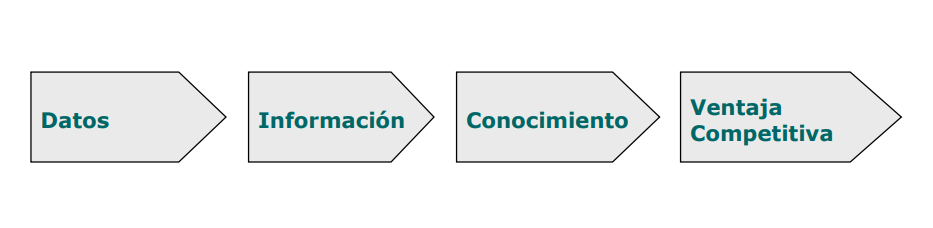
\includegraphics[width=7cm]{./Imagenes/bi} 
\end{center}

\item Analisis de Negocio (BA): \\ 
El análisis de negocio es el conjunto de métodos y técnicas utilizadas para trabajar como enlace entre los stakeholders con el fin de comprender la estructura, políticas y operaciones de una organización y recomendar soluciones que permitan alcanzar sus objetivos. El análisis de negocio implica la comprensión de cómo funcionan las organizaciones para llevar a cabo sus propósitos y la definición de las capacidades que requiere para proporcionar productos y servicios a los grupos de interés externos.

\end{itemize}



%----------------------------------------------------------------------------------------
%	DESARROLLO
%----------------------------------------------------------------------------------------

\section{Desarrollo}

\subsection{¿En que se diferencian Business Intelligence con Business Analytics?}
La diferencia principal en ambas ideas es que el Business Inteligence se enfoca en los datos que manejamos los datos ya recopilados la cual la podemos convertir en informacion
y usarla para analizarlas y entender el pasado del negocio. Por otro lado el Business Analytics nos permitira centrarnos en el presente para crear una vision clara del futuro y predecir (mediante modelos predectivos) para adelantarnos al futuro.

\subsection{¿En que se asemejan Business Intelligence con Business Analytics?}

NOSE SOLO EN RECOPILAR LA INFORMACION :V HAGAN P



%----------------------------------------------------------------------------------------
%	CONCLUSIONES
%----------------------------------------------------------------------------------------

%----------------ESTO LO HIZO EL OTRO TEAMMMMMM :v :V -----------------------------------------------------------------------
%----------------ESTO LO HIZO EL OTRO TEAMMMMMM :v :V -----------------------------------------------------------------------
%----------------ESTO LO HIZO EL OTRO TEAMMMMMM :v :V -----------------------------------------------------------------------
%----------------ESTO LO HIZO EL OTRO TEAMMMMMM :v :V -----------------------------------------------------------------------
%----------------HAY QUE CAMBIARLO -----------------------------------------------------------------------
%----------------HAY QUE CAMBIARLO -----------------------------------------------------------------------
%----------------HAY QUE CAMBIARLO -----------------------------------------------------------------------
%----------------HAY QUE CAMBIARLO -----------------------------------------------------------------------


\section{Conclusiones}
\begin{itemize}	

	\item  En el mundo empresariial, las empresas tienen un area que brinda soporte a los procesos de informacion, estrategia, lo que los lleva a un mercado competitivo, la inteligencia de negocios para una empresa la hace una pieza fundamenta a la hora de tomar mejores deciones.
	\item El numero creciente de pequeñas y medianas empresas da una notoria cifra sobre la ausencia de un sistema de inteligencia empresarial para la gestion de sus empresas. Pero en contraste si tienen conocimiento del concepto y de sus beneficios como el del acceso a datos criticos de la empresa, oportunidades competitivas, tomar mejores deciciones, etc.
	\item Lo que buscan estas herramientas es fomentar la exploración de datos y la toma de decisiones basadas en hechos.
	\item El Business analytics busca prodocir conocimiento estadisticoos y matematicos a partir de datos, con el objetico de generar probales escenarios y opciones con las que lidiar, a comparacion del Business Intelligence que proporciones un analisis a base de datos historicos

\end{itemize} 



%----------------------------------------------------------------------------------------
%	BIBLIOGRAFIA
%----------------------------------------------------------------------------------------


\begin{thebibliography}{99} 

\bibitem[Silvia Chavez y Carmen Contreras, 2018]{}
\newblock Implementación de Business Intelligence, para el proceso de toma de decisiones del área de ventas.

\bibitem[Hans Peter Luhn 1958]{}
\newblock A Business Intelligence System

\bibitem[Alex Rayón, 2015]{Universidad de Deusto}
Conceptos básicos del Business Intelligence.

\bibitem[Jordi Conesa y Josep Curto, 2010]{}
\newblock Introduccion al Business Intelligence

\bibitem[Margaret Rouse, 2019]{}
\newblock Análisis de negocios (BA)

\bibitem[Noodle Editorial Staff, 2018]{}
\newblock Business analytics career paths

\bibitem[Josep Lluis Cano, 2007]{}
\newblock Business Intelligence: competir con información


\bibitem[Curto J., 2010]{} 
\newblock Introducción al Business Intelligence. Editorial UOC.

\bibitem[Kimball R. and Ross M., 2002]{} 
\newblock  The Data Warehouse Toolkit: The Complete Guide to Dimensional Modeling. Wiley

\bibitem[Carolina A., 2017]{} 
\newblock  Análisis de Negocio (Business Analysis, BA)
 
\end{thebibliography}


%----------------------------------------------------------------------------------------


\end{document}
